\documentclass[9pt,twocolumn,twoside]{pnas-report}

\usepackage{todonotes}

\setuptodonotes{inline,size=\small,color=blue!40}

\templatetype{pnasresearcharticle}

\usepackage{lipsum}


% set figures directory to be ./figures
\graphicspath{{./figures/}}

\title{\textcolor{red}{Draft} Security Analysis of Open-Source Software Package Ecosystems}

\author[a]{Žiga Trček}
\author[a]{Matej Urbas}
\author[a]{Jan Vasiljević}

\affil[a]{University of Ljubljana, Faculty of Computer and Information Science, Ve\v{c}na pot 113, SI-1000 Ljubljana, Slovenia}

\leadauthor{Jan Vasiljević}

\authordeclaration{All authors contributed equally to this work.}
\correspondingauthor{\textsuperscript{1}To whom correspondence should be addressed. E-mail: fine.author@email.com.}

\begin{abstract}
The use of open-source packages and libraries significantly accelerates software development but simultaneously introduces numerous security risks.
Motivated by a recent near-compromise of OpenSSH by a malicious actor, this study aims to investigate the security of open-source software by conceptualizing it as a network and examining transitive vulnerabilities.
Our analysis specifically focuses on PyPI, npm, and crates.io, which are the predominant package managers for Python, JavaScript, and Rust, respectively.
Through this exploration, we seek to uncover potential security weaknesses within these ecosystems and propose methods to enhance their security posture.

\todo{Ni se koncano: Cakam da mamo dejansk neki narejeno. Bolj placeholder.}
\end{abstract}
	
\dates{The manuscript was compiled on \today}
\doi{\href{https://ucilnica.fri.uni-lj.si/course/view.php?id=183}{Introduction to Network Analysis} 2023/24}

\begin{document}

\maketitle
\thispagestyle{firststyle}
\ifthenelse{\boolean{shortarticle}}{\ifthenelse{\boolean{singlecolumn}}{\abscontentformatted}{\abscontent}}{}

\dropcap{T}he date is March 28, 2024. A principal software engineer at Microsoft notices an unusual delay in his login attempts, timing at approximately 500ms—significantly longer than usual by his standards. This prompts an investigation into higher than normal CPU usage, during which he observes anomalous behavior in the SSH daemon process. This unexpected discovery leads to the identification of a vulnerability in the XZ Utils library utilized by OpenSSH. The breach, orchestrated by a malicious actor through a combination of social engineering, code injection, and obfuscation, was set into motion over several years. Interestingly, the core code of OpenSSH remained untouched; instead, a transitive dependency was exploited. Had this vulnerability remained undetected, it could have potentially compromised a vast number of servers relying on OpenSSH, embedding a remote code execution backdoor.


In a manner similar to the exploitation of the XZ Utils library, other open-source software packages and libraries are also vulnerable to malicious attacks.
The development of software inherently involves placing trust in the authors of utilized libraries, who are often individual hobbyists or small teams with limited resources.
The potential for significant damage is large if a malicious actor targets a lesser-maintained package that, while small, is widely used—either directly or as a transitive dependency in other software projects.
The incident involving the left-pad package, which was removed from npm and consequently led to the failure of numerous dependent packages, serves as a reminder of the inherent fragility within the open-source ecosystem.

Int this project we look at three different pacakge ecosystems: PyPI, npm, and crates.io, which are package repositories for Python, JavaScript, and Rust, respectively. We aim to investigate the security of these ecosystems by conceptualizing them as networks.... \textcolor{red}{Zej ne bom pisal dokler ne dejansko necesa nardimo.}

\todo{Problem definition, motivation, background, contributions etc. + Mandatory informative illustration highlighting main contributions}


\section*{Related work}

Robustness of dependency networks is a topic that has been examined in several studies.
\cite{hafner2021robustness} explored the robustness of the npm package dependency network and highlighted its vulnerability to targeted attacks by identifying crucial nodes.
Attacks on such nodes could gravely affect a large portion of the network, as they are responsible for a significant number of dependencies.
Their findings suggest that while the network has crucial nodes, it is not highly vulnerable as they are mostly large and well-maintained projects.
Moreover, the network is trending towards a more robust state, as the number of dependencies is decreasing over time.

\cite{decan2018evolution} published a comparative analysis of dependency networks across 7 package ecosystems, including Cargo, CPAN, CRAN, npm, NuGet, Packagist, and RubyGems.
They proposed metrics to capture growth, changeability, reusability, and fragility.
They revealed that while the ecosystems are growing, a minority of packages are responsible for most updates and dependencies.
Furthermore, it is suggested that even transitive dependencies on unmaintained or obsolete packages can have a detrimental effect on the security and maintainability of the ecosystem.

\cite{tsakpinis2024accessibility} carried out a study on the accessibility of GitHub repositories for npm and PyPI libraries to understand the level of maintenance for them.
Their research showed that a significant portion of libraries lacked valid repository URLs, which hinders the ability to monitor vulnerabilities and maintain codebases.
An emphasis on the importance of maintaining valid repository URLs was made, as it is crucial for the sustainability of the open-source ecosystem.

Community detection has been proposed as a security analysis tool.
The found communities can provide great insight into the structure of the network and the relationships between packages, which helps assess the robustness of the network.
Understanding what packages are closely related and how they are connected can help identify potential vulnerabilities and dependencies that could be exploited by attackers \cite{hafner2021robustness, tsakpinis2024accessibility}.

\cite{korkmazrpackages} examine the dependency graph of R packages and the relationship between various metrics.
They find that centrality measures have a high correlation with the number of downloads and citations of a package.
Furthermore, package attributes such as number of authors and commits also have a positive impact on the number of downloads and citations.

Security vulnerability data analysis has been a large area of research in the recent years.
\cite{decan2018vulnerabilities} studied around 400 security reports from the npm network to understand how they are discovered and fixed, and how they affect the network.
They found that it takes around a year for a discovered vulnerability to be published publically, while it takes around 2 years after the discovery for the vulnerability to be fixed.
\cite{shahzad2012} study vulnerability life cycles on a large software vulnerability dataset, getting similar results.

\cite{HANIF2021103009} propose and evaluate novel machine learning approaches to vulnerability prediction in open-source software.
Some simple vulnerabilities are easily detected by their approach, but even more complex vulnerabilities can be detected with high accuracy.

\cite{hejderup2018} use call graphs instead of dependency graphs to detect dependencies in software.
They find that call graphs are efficient in aiding preliminary evaluation of security issues and their impact to other applications.
Furthermore, \cite{hejderup2022prazi} find that Cargo packages call only 40\% of their dependencies, which can lead to many unneeded security vulnerabilities.

\cite{ruohonen2021} examine around 200000 PyPI packages using static analysis and find that around 46\% of the packages have at least one security vulnerability.

\section*{Results}

 {\bf Main results supported by math, plots, tables, diagrams etc.}
\lipsum[1]

\begin{table}[h]\centering%
	\caption{Table describing data or methods.}
	\begin{tabular}{lccccc}\toprule
		             & $n$        & $m$           & $\langle k\rangle$ & $\langle C\rangle$ & $\langle d\rangle$ \\\midrule
		Fine network & $438\,920$ & $9\,742\,733$ & $44.4$             & $0.37$             & $6.19$             \\
		Random graph & $438\,920$ & $9\,781\,609$ & $44.6$             & $0.00$             & $4.92$             \\\bottomrule
	\end{tabular}
	\label{tbl:example}
\end{table}

\lipsum[2-3]

\begin{figure}[t]\centering%
	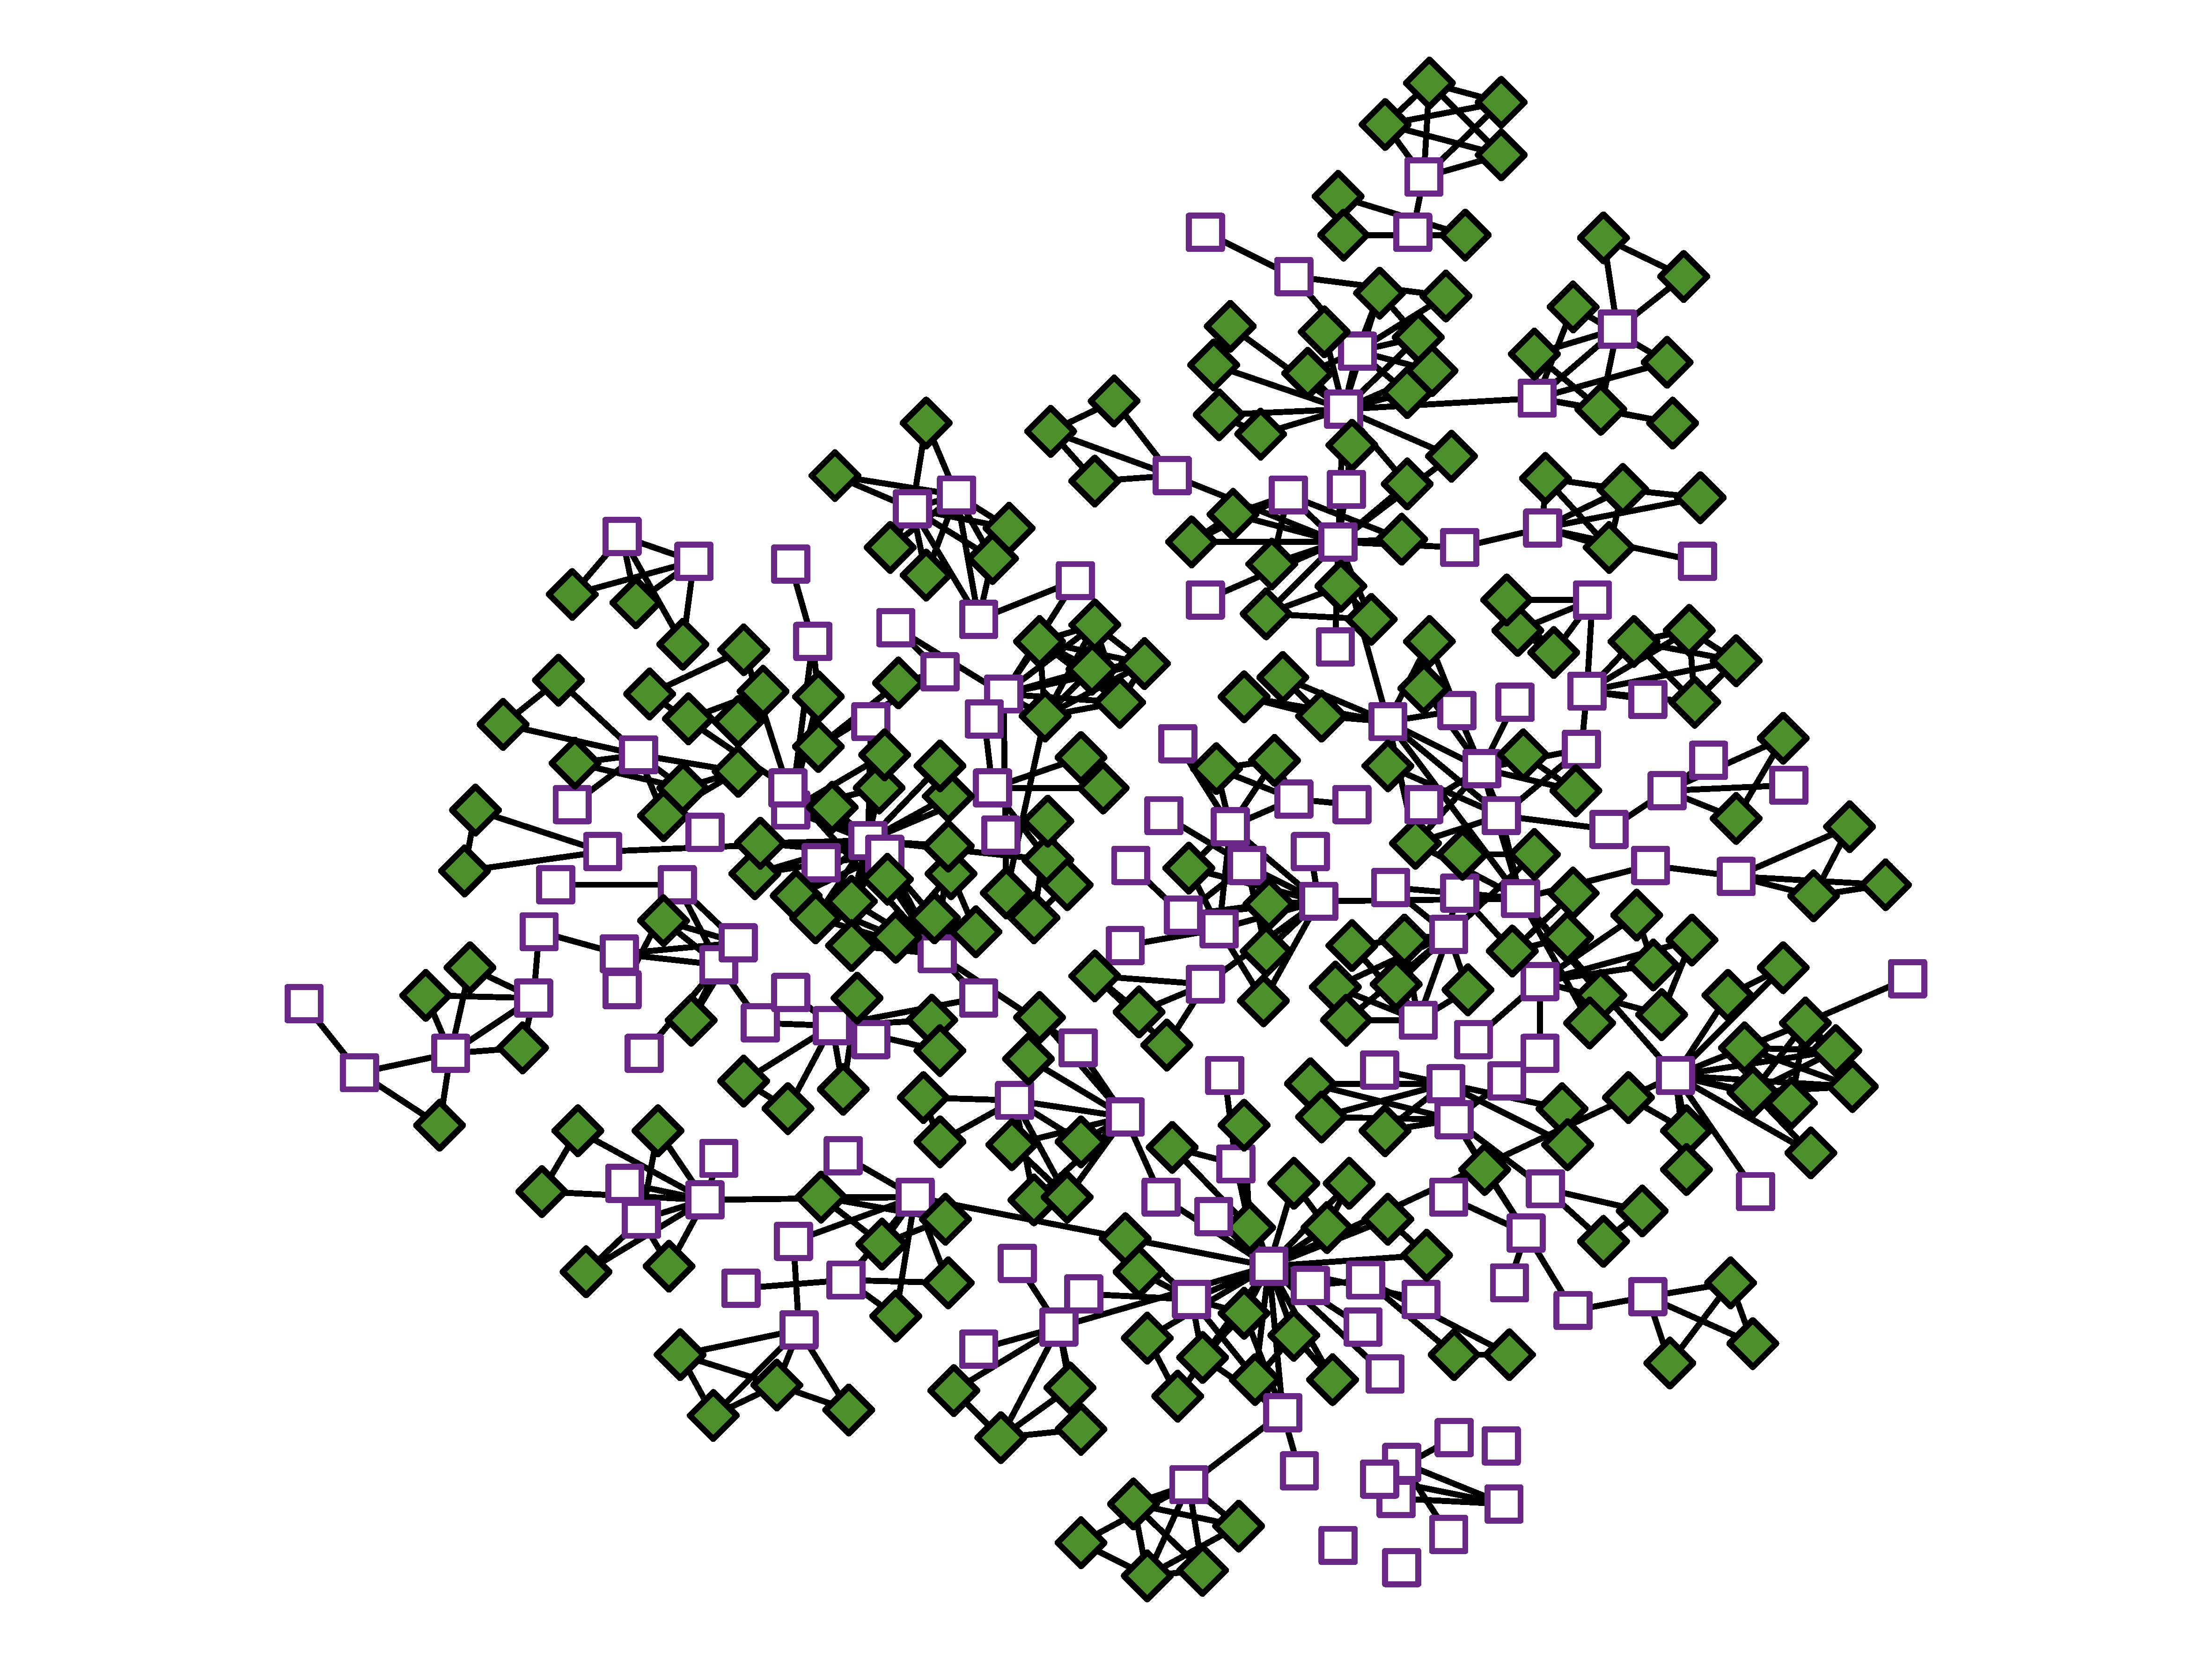
\includegraphics[width=0.49\linewidth]{example1}
	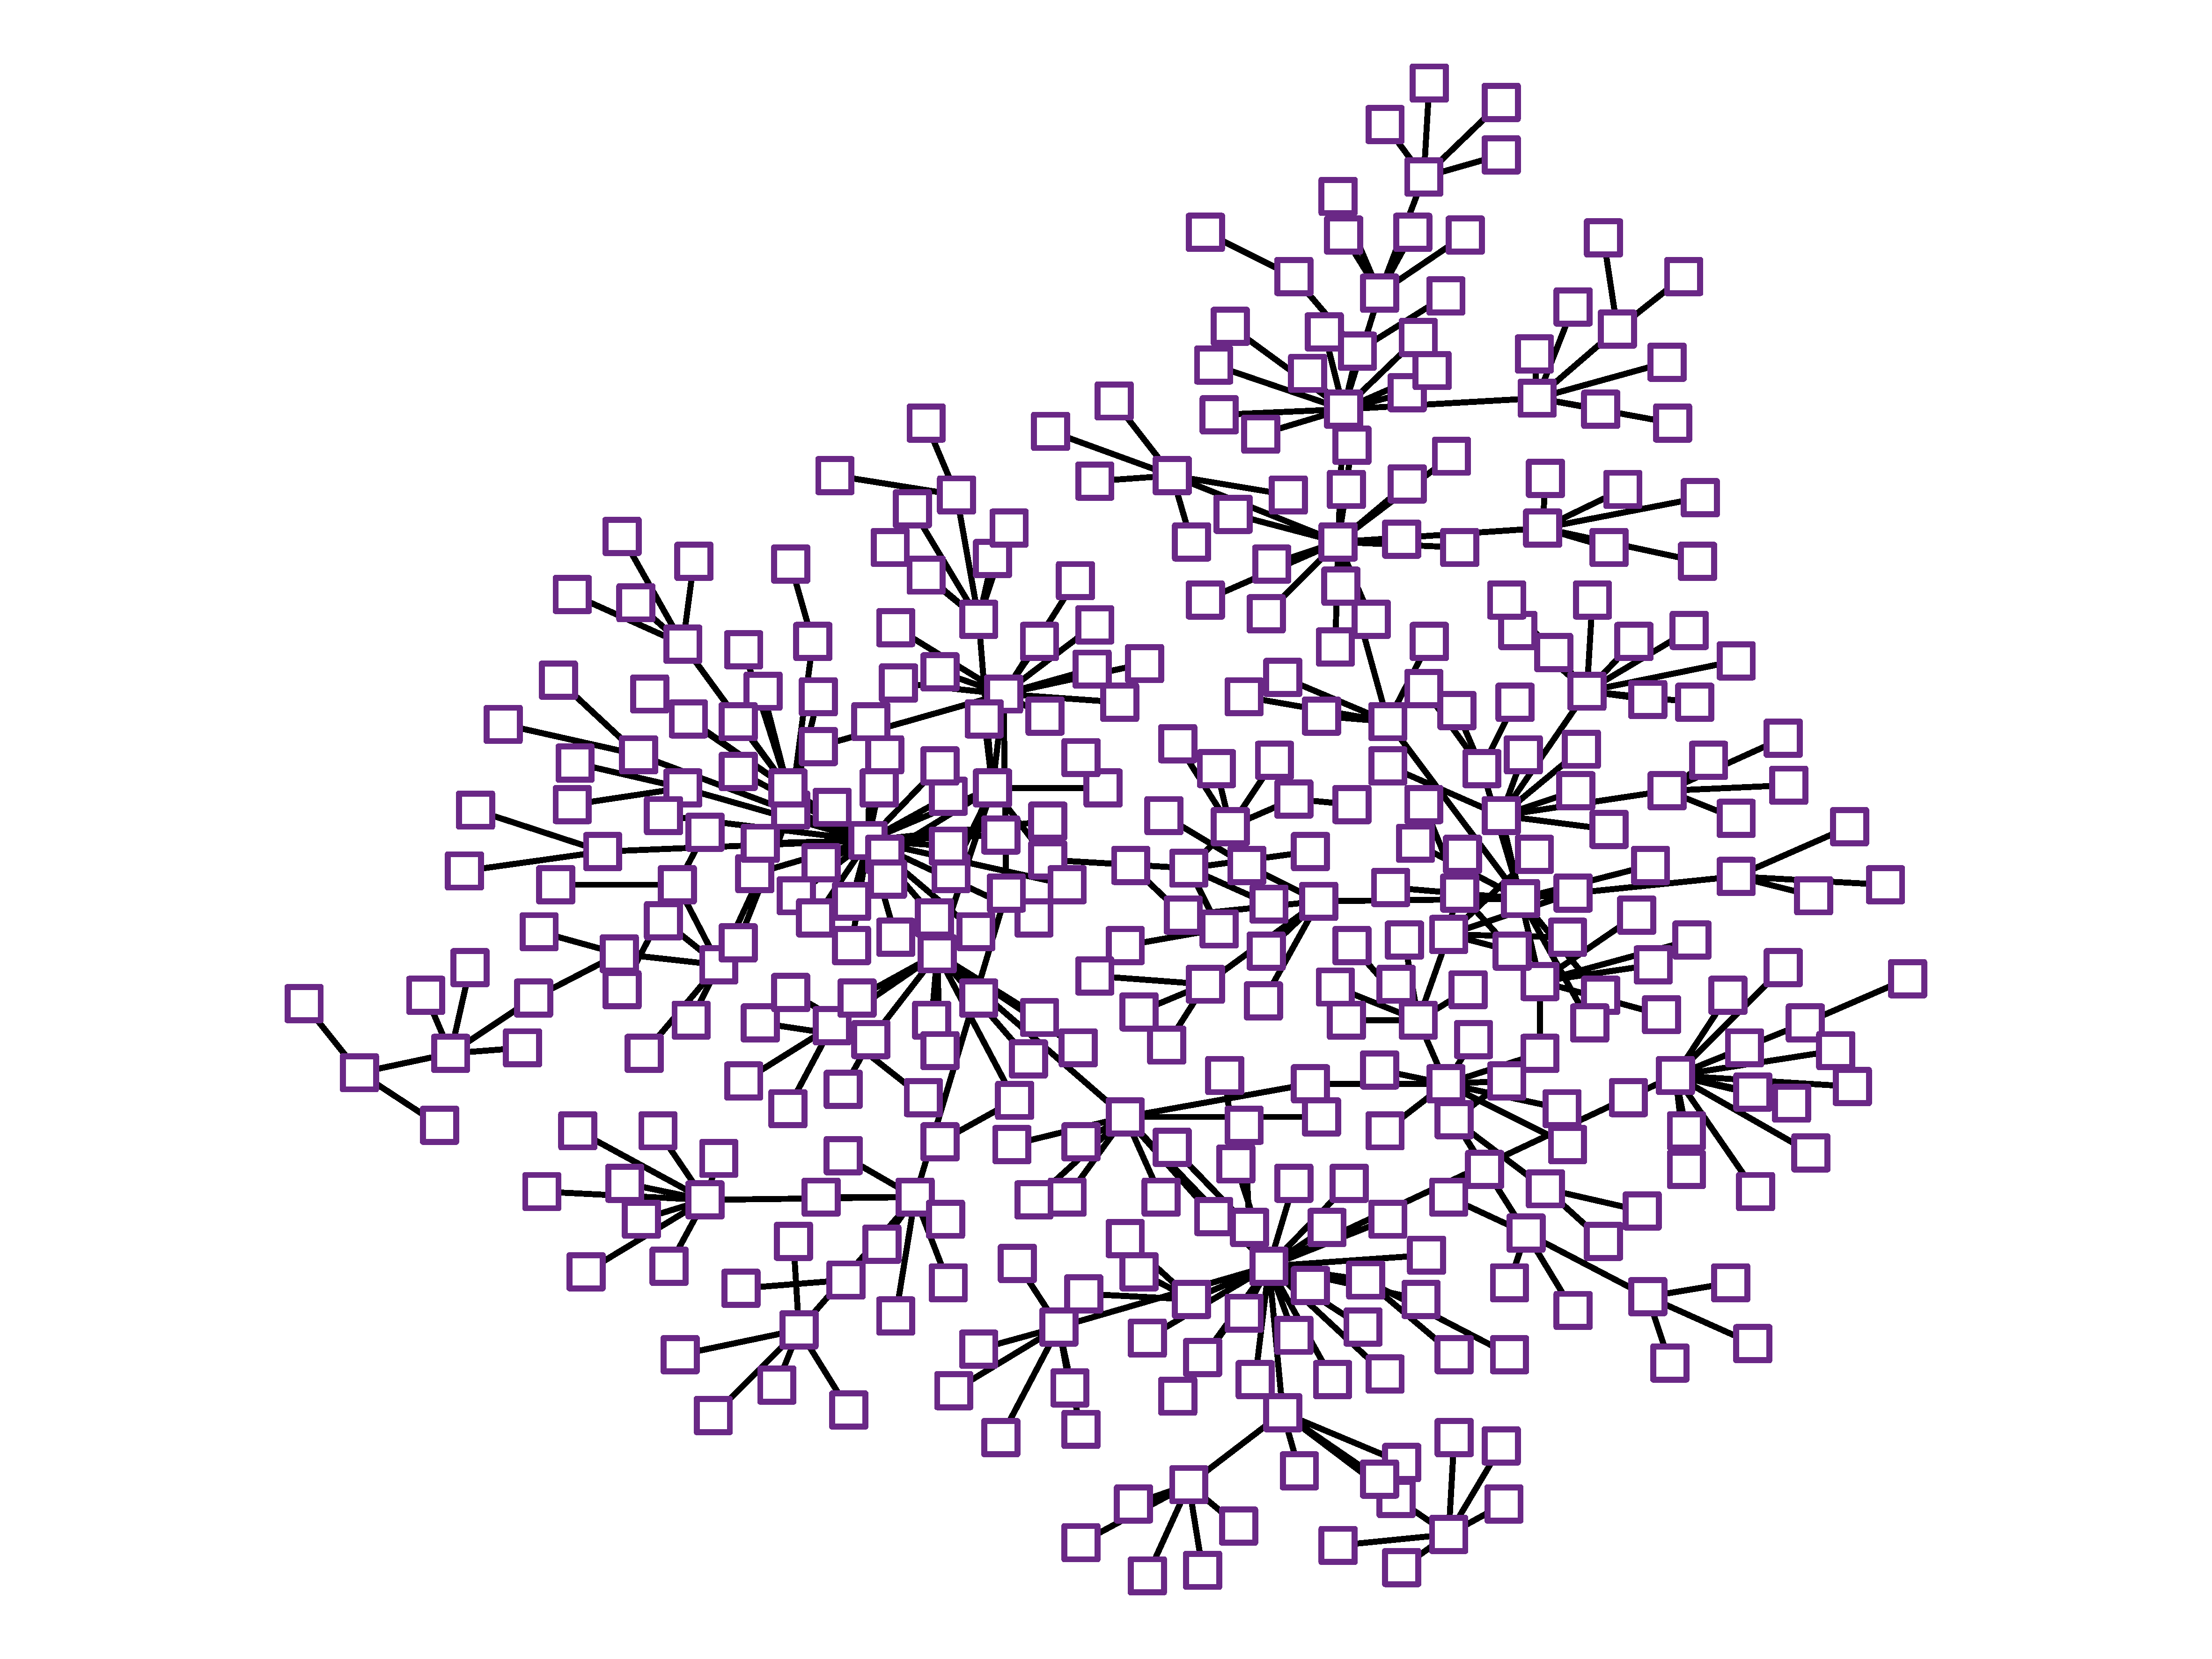
\includegraphics[width=0.49\linewidth]{example2}
	\caption{Figure showing interesting examples.~\cite{Sub18a}}
\end{figure}

\lipsum[4-6]

\begin{figure}[b]\centering%
	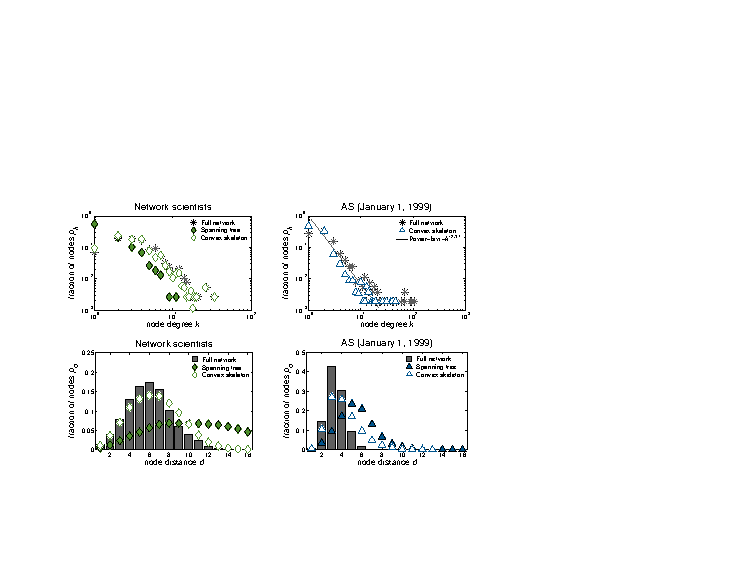
\includegraphics[width=\linewidth]{distributions}
	\caption{Figure showing relevant results.~\cite{Sub18a}}
\end{figure}

\begin{figure}[t]\centering%
	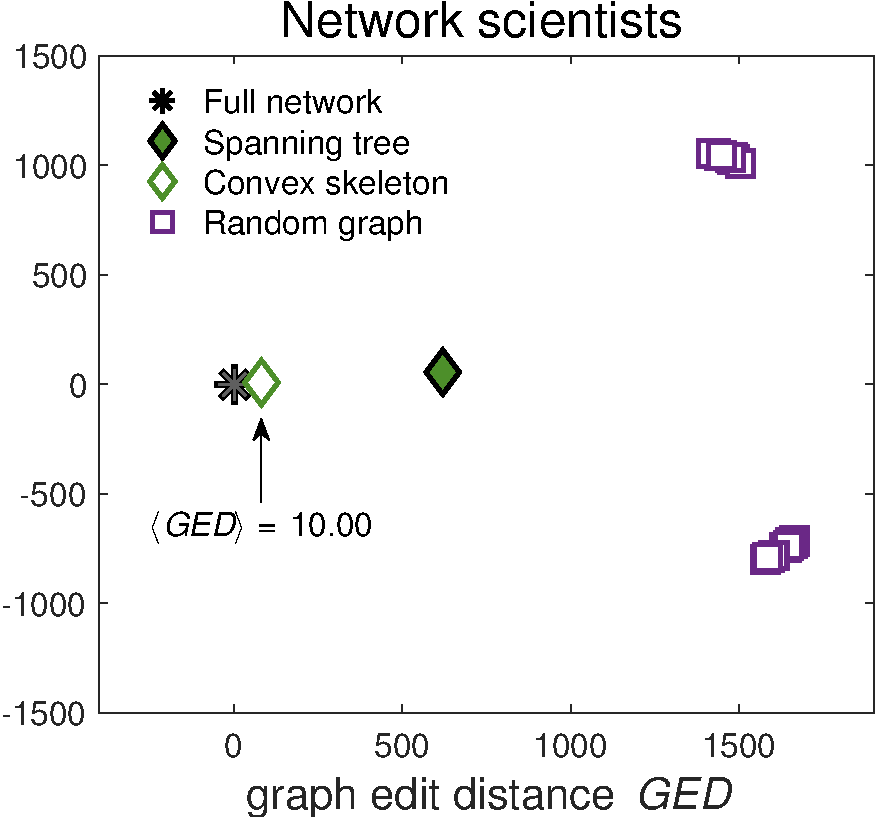
\includegraphics[width=0.45\linewidth]{results1}\hskip12pt
	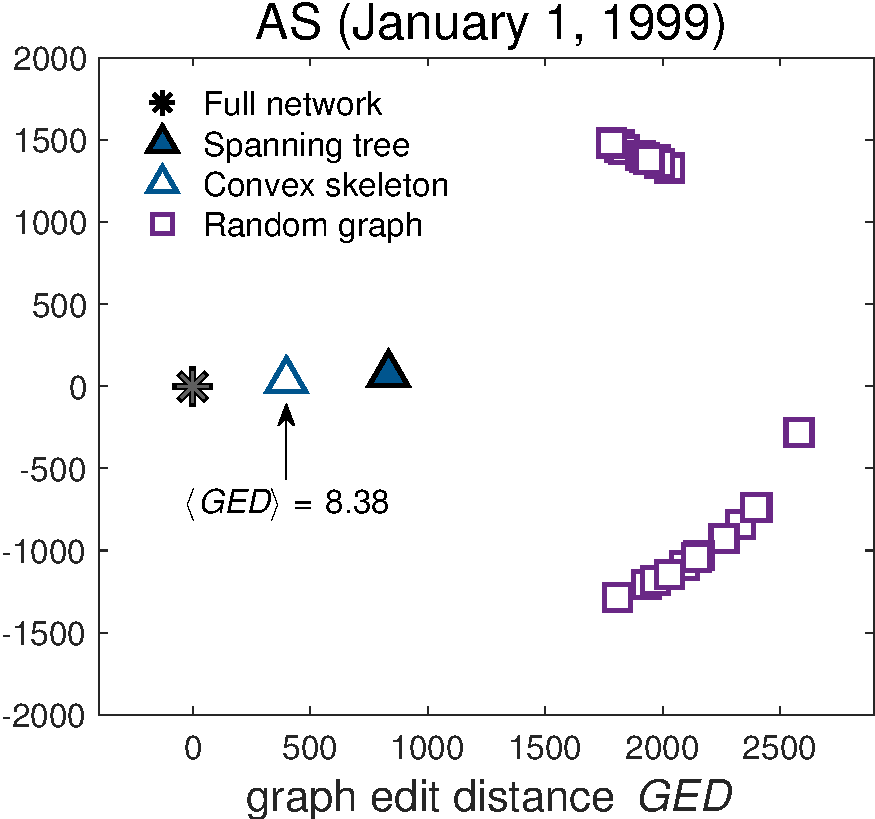
\includegraphics[width=0.45\linewidth]{results2}
	\caption{Another figure with results.~\cite{Sub18a}}
	\label{fig:example}
\end{figure}

\section*{Discussion}

 {\bf Summary of results, main contributions, final conclusions, future work etc.}
\lipsum[1-3]

\small

\section*{Methods}

 {\bf Data, methods, algorithms etc.}
\lipsum[1]

\begin{equation}
	\phi_v = \Pr(X_{st}(v) = 1) = \Pr(X_{sv} = 1)\Pr(X_{vt} = 1)
	\label{eq:example}
\end{equation}

\lipsum[2]

\begin{algorithm}[H]
	\begin{algorithmic}[1]
		\Require graph $G$, cutoff $k_{min}$
		\Ensure power-law $\gamma$
		\State $s\gets$ $n\gets$ $0$
		\For{nodes $i\in N$}
		\If {$k_i\geq k_{min}$}
		\State $s\gets$ $s+\ln k_i/(k_{min}-0.5)$
		\State $n\gets$ $n+1$
		\EndIf
		\EndFor
		\State \Return $1+ns^{-1}$
	\end{algorithmic} \vspace{8pt}
\end{algorithm}

\lipsum[3-4]

\normalsize

% \acknow{The authors would like to\dots}

% \showacknow{}

\bibliography{bibliography}

\end{document}
